% vim:spell:spelllang=en

\input defs.tex



% \newcommand{\domzone}[1]{\mathit{dom}({#1})}
% \newcommand{\sdomzone}[1]{\mathit{sdom}({#1})}
% \newcommand{\ldef}[1]{#1}
% \newcommand{\luse}[1]{\mathit{uses}\,#1}
% \newcommand{\DF}[1]{\mathrm{DF}_{#1}}
% \newcommand{\IDF}{\mathrm{DF}^+}
% \newcommand{\JS}[1]{\mathcal{J}_{#1}}
% \newcommand{\IJS}{\JS{\infty}}
% \newcommand{\nepath}[2]{{#1}{\overset{+}{\rightarrow}}{#2}}

\title{SSA Reconstruction}
\author{Sebastian Hack}

\chapter{SSA Reconstruction \Author{S. Hack}}
% \numberofpages{6}

\section{Introduction}

Some optimizations break the single-assignment property of the SSA form by inserting additional definitions for a single SSA value.
A common example is live-range splitting by inserting copy operations or inserting spill and reload code during register allocation.
Other optimizations, such as loop unrolling or jump threading, perform similar operations.
Let us first go through two examples before we present algorithms to repair SSA.

\subsection{Live-Range Splitting}

In Figure~\ref{fig:nonssa}, our spilling pass decided to spill a part of the live range of the variable~$x_0$ in the right block.
Therefore, it inserted a store and a load instruction. 
The load however is a second definition of $x_0$, hence SSA is violated and has to be reconstructed as shown in Figure~\ref{fig:recons}.

\begin{figure}[htbp]
	\centering
	\subfigure[Original program] {
		\label{fig:harmless}
		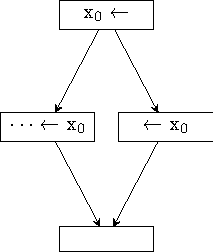
\includegraphics{spill_orig.pdf}
		% \input spill_orig.tikz
	}
	\hfill
	\subfigure[Spilling~$x_0$, SSA violated] {
		\label{fig:nonssa}
		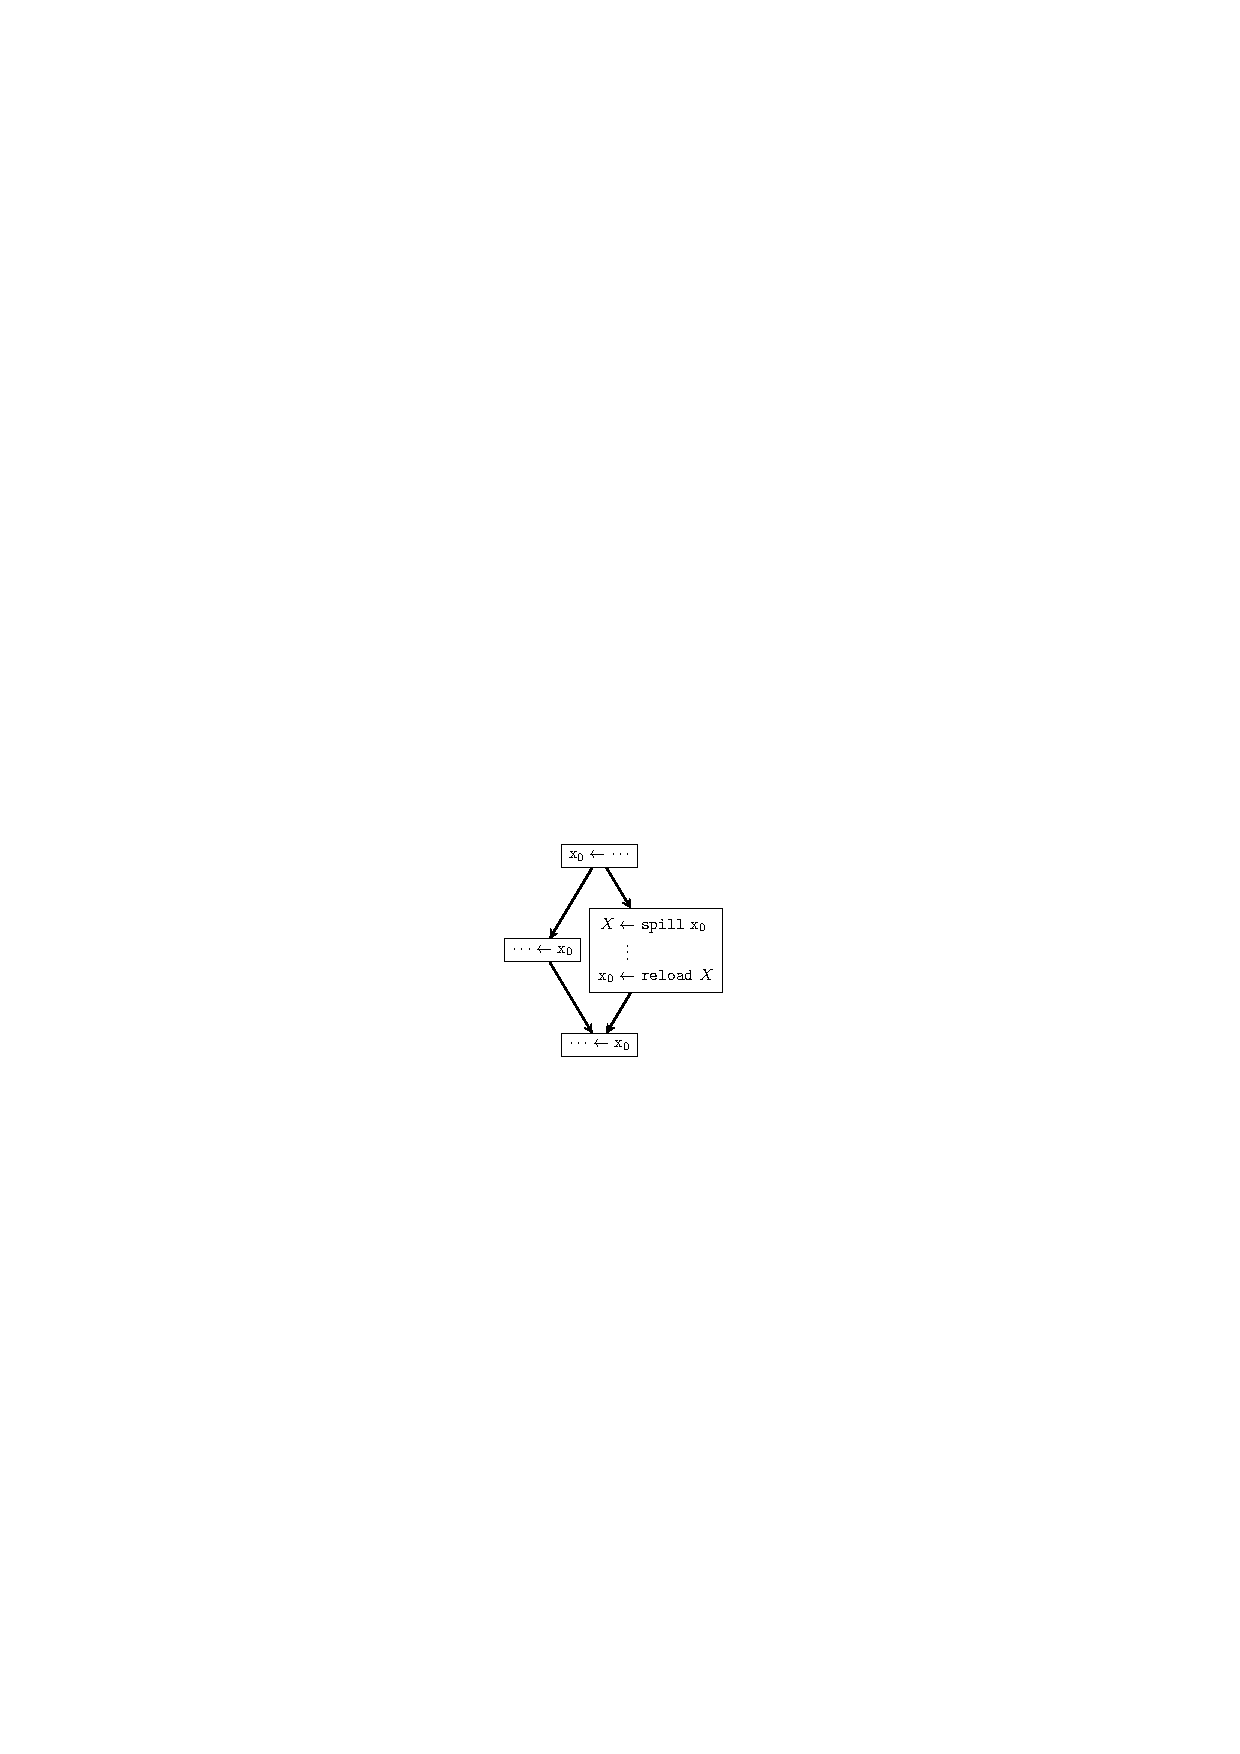
\includegraphics{spill_nonssa.pdf}
	}
	\hfill
	\subfigure[SSA reconstructed] {
		\label{fig:recons}
		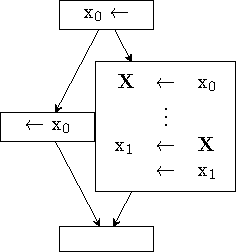
\includegraphics{spill_recons.pdf}
	}
	\label{fig:ex1}
	\caption{Adding a second definition}
\end{figure}

In a more complicated configuration, adding a second definition to an SSA variable can cause \phiops\ to be inserted.
Figure~\ref{fig:withphis} shows the same program fragment with the left use of~$\var x_0$ being moved to the bottom.
As there are two definitions reaching the use in the lower block, a \phiop\ has to be inserted. 

\begin{figure}[htbp]
	\centering
	\subfigure[Original program] {
		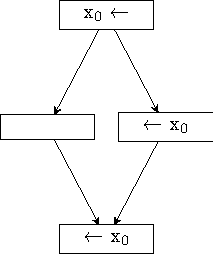
\includegraphics{spill_phi_orig.pdf}
	}
	\phantom{XXX}
	\subfigure[Second definition of~$\var x_0$, \phiop\ inserted] {
		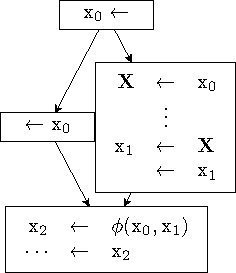
\includegraphics{spill_phi.pdf}
	}
	\label{fig:withphis}
\end{figure}

Such program modifications are done by many optimizations. 
Not surprisingly, maintaining SSA is often one of the more complicated and error-prone parts in such optimizations;
owing to the insertion of additional \phiops\ and the correct redirection of the variable's uses.

\subsection{Loop Unrolling}

Loop unrolling is a transformation to increase instruction-level parallelism inside the body of a loop.
To this end, the body of the loop is duplicated $n$~times. 
Similar to the example above, this adds several new definitions \emph{and} uses to an existing SSA variable. 
Consider following example and assume that the loop's body is duplicated once, i.e.~the loop is unrolled once.

\begin{figure}[htbp]
	\begin{center}
		\subfigure[Original loop] {
			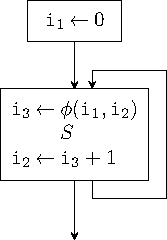
\includegraphics{loop_orig.pdf}
		}
		\phantom{XXX}
		\subfigure[Unrolled loop, code duplicated, SSA broken] {
			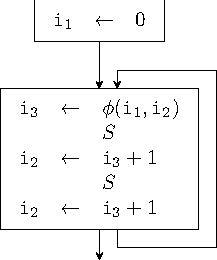
\includegraphics{loop_unroll.pdf}
		}
		\phantom{XXX}
		\subfigure[SSA repaired] {
			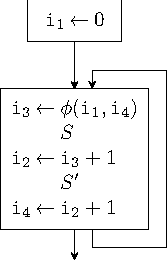
\includegraphics{loop_unroll_repair.pdf}
		}
	\end{center}
	\caption{Loop Unrolling}
	\label{fig:unroll}
\end{figure}

These examples show that naive code duplication and live-range splitting in an SSA program can violate the single assignment property of the SSA form.
To repair these effects, we seek for a simple, black box like algorithm.
Ideally, we provide a set of definitions and uses of which we claim that they correspond to one single non-SSA variable.
Afterwards, the algorithm establishes the SSA form for these live ranges.
This includes re-assigning the uses to the correct definition and inserting \phiops\ on demand.
Next, we investigate an algorithm based on the classical dominance frontier construction algorithm.

\section{Reconstruction based on the Dominance Frontier}
After spilling, the program must be in SSA form to benefit from the results of Section~\ref{sec:core}.
However, if a variable $v$ is reloaded at several locations, these reloads form additional definitions of $v$.
This clearly violates the static single assignment property (see Figure~\ref{fig:spill_ssa}).
Therefore, for each variable $v$ for which reloads are introduced by the spiller, SSA has to be reconstructed.

Instead of performing an SSA construction algorithm on the whole program, we can restrict ourselves to the variables which were involved in spilling. All other variables still have only one definition.

We follow the same principles as the classical SSA construction algorithm by \cite{cytron:1991:ssa}:
For each spilled variable $x$ compute the iterated dominance frontier of the set of labels $L$ containing the definition and all labels containing a reload of $x$:
% \[L=\{\ell\mid \lres(\ell)=\{x\}\wedge\lop(\ell)=\spld\}\cup\{\ldef{x}\}\]
Firstly, give each variable defined by the labels in $L$ a new version number.
This reinstalls the single assignment property. Secondly, we have to rewire each use of former $x$ to one of the variables defined at the labels in $L$. 
Let $F$ bet the set of iterated dominance frontiers of $L$ (for example, see \cite[page 406]{appel:2002:modern} for an algorithm to compute these).
Let $U$ be the set of uses of $x$.
For each $\ell\in U$ we search up the dominator tree.
If we reach a label $\ell_r$ in $L$, we subsitute $x$ in $larg(\ell)$ by $lres(\ell_r)$.
If $\ell$ is in the iterated dominance frontier $F$, we insert a \phiop\ and search the predecessors of $\ell$ for valid definitions of $x$.
Algorithm~\ref{alg:ssaconstr} shows this procedure in pseudo-code.
Note that by re-wiring the usages of several variables, some variables defined by \phiops\ may not be used anymore.
A dead code elimination pass after spilling will remove these. 

\begin{algorithm}
  \caption{SSA reconstruction}
  \label{alg:ssaconstr}

\begin{verbatim}
proc ssa_reconstruct(variable v, set of program points d):
  f = iterated dominance frontier(union(def(v), d))
  for each use u of v:
    x = find_def(u)
    rewrite 
  end
end

proc find_def(var l, int i, set of var D, set of var F)
  if u == phi:
    l = pred(l, i)
  while i != root:  # while not at the root of the CFG
    if l in D:      # l is a definition of the variable
      return l
    elsif l in F:   # l is in the dom front of the variable's definitions
      insert new phi function p = phi()
      for i in 0 ... #preds: 
        d = find_def(p, i, D, F)
        set i-th operand of p to d
	  return p
    else:
      l = idom(l)
\end{verbatim}
\end{algorithm}



\section{Search-based Reconstruction}

The second algorithm we present here is based on Cliff Click's SSA construction algorithm (TODO: cite).
Although this algorithm is designed to construct SSA from the abstract syntax tree, it also works well on control flow graphs if one obeys certain rules.
Its major advantage over the algorithm presented in Section~\ref{sec:df} is that it does neither require dominance information nor dominance frontiers.
Thus it is well suited to be used in transformations that change the control flow graph.
The principle idea is to start a depth-first search from every use to find the corresponding definition inserting \phiops\ on the fly. 



